\documentclass[12pt, twoside]{article}
\documentclass[12pt, twoside]{article}
\usepackage[letterpaper, margin=1in, headsep=0.2in]{geometry}
\setlength{\headheight}{0.6in}
%\usepackage[english]{babel}
\usepackage[utf8]{inputenc}
\usepackage{microtype}
\usepackage{amsmath}
\usepackage{amssymb}
%\usepackage{amsfonts}
\usepackage{siunitx} %units in math. eg 20\milli\meter
\usepackage{yhmath} % for arcs, overparenth command
\usepackage{tikz} %graphics
\usetikzlibrary{quotes, angles}
\usepackage{graphicx} %consider setting \graphicspath{{images/}}
\usepackage{parskip} %no paragraph indent
\usepackage{enumitem}
\usepackage{multicol}
\usepackage{venndiagram}

\usepackage{fancyhdr}
\pagestyle{fancy}
\fancyhf{}
\renewcommand{\headrulewidth}{0pt} % disable the underline of the header
\raggedbottom
\hfuzz=2mm %suppresses overfull box warnings

\usepackage{hyperref}
\usepackage{float}

\fancyhead[LE]{\thepage}
\fancyhead[RO]{\thepage \\ First and last name: \hspace{2.5cm} \,\\ Section: \hspace{2.5cm} \,}
\fancyhead[LO]{BECA/Huson/Geometry: Trigonometry \\* 31 January 2025}

\begin{document}
\subsubsection*{4.14 Exam: Trigonometry and Cumulative Review}
\begin{enumerate}[itemsep=0.5cm]
\item Point $G$ bisects $\overline{FH}$, with $FG=5x + 7$, $GH=22$. Find $x$. \par \medskip
  \begin{tikzpicture}
      \draw[fill] (0,0) circle [radius=0.05] node[below]{$F$};
      \draw[-, thick] (0,0)--(8,0);
      \draw[fill] (4,0) circle [radius=0.05] node[below]{$G$};
      \draw[fill] (8,0) circle [radius=0.05] node[below]{$H$};
      \node at (2,0.5) [above]{$5x + 7$};
      \node at (6,0.5) [above]{$22$};
      \draw (1.8,-0.2)--(1.9,0.2);
      \draw (2.1,-0.2)--(2.2,0.2);
      \draw (5.8,-0.2)--(5.9,0.2);
      \draw (6.1,-0.2)--(6.2,0.2);
  \end{tikzpicture} \vspace{2cm}

\subsubsection*{G.CO.12 Make and justify formal geometric constructions}
\item Construct a perpendicular bisector of $\overline{PQ}$.  
  \vspace{1cm}
  \begin{center}
  \begin{tikzpicture}
    \draw [-, thick] (0,0)--(2,-4);
    \draw [fill] (0,0) circle [radius=0.05] node[above]{$P$};
    \draw [fill] (2,-4) circle [radius=0.05] node[below]{$Q$};
  \end{tikzpicture}
  \end{center} 
  \vspace{1cm}

\item Construct the angle bisector of $\angle A$.  
  %\vspace{1cm}
  \begin{center}
  \begin{tikzpicture}
    \draw [<->, thick] (6,3)--(0,0)--(6,-2);
    \draw [fill] (0,0) circle [radius=0.05] node[below left]{$A$};
  \end{tikzpicture}
  \end{center} 
  %\vspace{3cm}
      
\newpage
\subsubsection*{G.CO.5 Transform a figure using translation, reflection, or rotation}
\item  Reflect $\triangle ABC$ across the $x$-axis. Label the image $\triangle A'B'C'$ on the graph.
    \begin{center}
      \begin{tikzpicture}[scale=0.6]
        \draw [help lines] (-8,-7) grid (8,7);
        \draw [thick, <->] (-8.4,0) -- (8.4,0) node [below right] {$x$};
        \draw [thick, <->] (0,-7.4)--(0,7.4) node [left] {$y$};
        \draw [thick] (0,2) node[left] {$A$}--
          (6,0) node[above right] {$B$}--
          (3,5) node[above right] {$C$}--
          cycle;
      \end{tikzpicture}
      \end{center}
  
\item A translation maps $P(2,3) \rightarrow P'(-5,0)$. What is the image of $Q(6,2)$ under the same translation? \vspace{1cm}
      
\item The translation mapping $x \rightarrow x+4$ and $y \rightarrow y - 5$ is applied to $\triangle ABC$.
  \begin{enumerate}
    \item Write as coordinate pairs the vertices of the image, $\triangle A'B'C'$ \\[0.3cm]
    $A(-1,2) \rightarrow$ \\[0.7cm]
    $B(3,-2) \rightarrow$ \\[0.7cm]
    $C(0,1) \rightarrow$ \\[0.1cm]
    \item Which triangle is larger, or are they the same size? Justify your answer.
  \end{enumerate} \vspace{2cm}

\newpage
\item Apply a counter clockwise rotation of $90^\circ$ centered at the origin to $\triangle ABC$. Plot and label the image on the axes below.
  \begin{center}
    \begin{tikzpicture}[scale=.7]
      \draw [help lines] (-8,-7) grid (8,8);
      \draw [thick, <->] (-7.4,0) -- (8.4,0) node [right] {$x$};
      \draw [thick, <->] (0,-7.4)--(0,8.4) node [above] {$y$};
      \draw [thick]
        (2,4) node[above right] {$A$}--
        (2,-1) node[below] {$B$}--
        (7,-1) node[below] {$C$}--
        cycle;
    \end{tikzpicture}
  \end{center}

\item Dilate $\triangle ABC \rightarrow \triangle A'B'C'$ by a factor of $k=2$ centered at the origin, \\
$(x,y) \rightarrow (2x, 2y)$. Plot and label the image on the axes.
  \begin{center}
      \begin{tikzpicture}[scale=0.8]
      \draw [help lines] (-1,-2) grid (8,6);
      \draw [thick, <->] (-1.4,0) -- (8.4,0) node [right] {$x$};
      \draw [thick, <->] (0,-2.4)--(0,6.4) node [above] {$y$};  
      \draw [thick]
          (0,0) node[below left] {$A$}--
          (2,2) node[above left] {$B$}--
          (2, -1) node[below left] {$C$}--cycle;  
      \end{tikzpicture}
  \end{center}

\newpage
\subsubsection*{G.SRT.5 Use similarity criteria for triangles to solve problems}
\item Given $\triangle ABC \sim \triangle DEF$, $m\angle A=45^\circ$, and $m\angle F=110^\circ$. Find $m\angle D$. \vspace{4cm}


\item Two triangles are shown with $P$ the intersection of $\overline{AJ}$ and $\overline{BK}$.
\begin{multicols}{2}
  \begin{enumerate}
      \item What theorem can be used to justify $\angle APB \cong \angle JPK$?
      \item What angle must be congruent to $\angle J$ to prove $\triangle ABP \sim \triangle JKP$ by \emph{angle-angle similarity}? \vspace{3cm}
      \end{enumerate}
  \begin{tikzpicture}[rotate=-20, scale=1.4]
      \draw [thick]
        (-0.25,-1)node[below left]{$B$}--
        (0.5,2)node[left]{$K$}--
        (4,0)node[below left]{$J$}--
        (0,0)node[above]{$P$}--
        (-2,0)node[left]{$A$}--cycle;
    \end{tikzpicture}
  \end{multicols}
    \vspace{1cm}

\item A dilation maps $\triangle ABC \rightarrow \triangle ADE$. Given $AB=12$, $AC=14$, $BC=10$, $DE=25$. 
\begin{multicols}{2}
    Find the scale factor and side lengths:\\[0.5cm]
    $k=$\\[1cm]
    $AE=$\\[1cm]
    $AD=$\\[1cm]
    $BD=$\\
    \begin{flushright}
    \begin{tikzpicture}[scale=1.]
        \draw [thick]
        (0,0)node[below]{$A$}--
        (0:6)node[below]{$D$}--
        (30:8)node[above]{$E$}--cycle;
        \draw [thick]
        (0:2.4)node[below]{$B$}--
        (30:3.2)node[above left]{$C$};
        \node at (0:1.5)[below]{$12$};
        \node at (15:2.7)[right]{$10$};
        \node at (15:6.75)[right]{$25$};
        \node at (35:1.7)[above]{$14$};
    \end{tikzpicture}
    \end{flushright}
\end{multicols}\vspace{0.25cm}

    
\newpage
\item Triangle $ADE$ is drawn with $\overline{BC} \parallel \overline{DE}$, as shown. Given $AB=6$, $BC=9$, $AC=10$, and $BD=6$.
\begin{multicols}{2}
  \begin{enumerate}
    \item Find $DE$. \vspace{1.5cm}
    \item Find $AE$.
  \end{enumerate}

%Find $CE$, $AE$, and $DE$. Find and mark all of the angle measures of the triangle.\vspace{1cm}
    \begin{flushright}
        \begin{tikzpicture}[scale=0.6]
        \draw [thick]
        (0.5,1.5)node[left]{$B$}--
        (6.5,1.5)node[above right]{$C$}--
        (2,6)node[above]{$A$}--cycle;
        \draw [thick]
        (0.5,1.5)--
        (-1,-3)node[left]{$D$}--
        (11,-3)node[below left]{$E$}--(6.5,1.5);
        \node at (3,1.5)[below]{$9$};
        \node at (4.5, 4)[right]{$10$};
        \node at (0.6, 3.3)[above]{$6$};
        \node at (-0.7, -1)[above]{$6$};
        \end{tikzpicture}
    \end{flushright}
  \end{multicols} \vspace{1cm}

\item In the diagram below, the chords $\overline{AE}$ and $\overline{BD}$ intersect at $C$, with $\triangle ABC \sim \triangle DEC$.
\begin{multicols}{2}
  \begin{enumerate}

    \item $m\angle A = 70^\circ$ and $m\angle B = 85^\circ$.\\ 
    Find  $m\angle D$.
    \item $BC=10$, $CD=20$, and $CE=15$.\\ 
    Find $AC$. 
  \end{enumerate}

    \begin{center}
    \begin{tikzpicture}[scale=.6]
    \draw (0,0) circle[radius=5];
    \draw [thick]
    (20:5) node[right] {$A$}--
    (160:5) node[left] {$E$}--
    (210:5) node[left] {$D$}--
    (50:5) node[above right] {$B$}--cycle;
    \draw (75:1.8) node[above] {$C$};
    \end{tikzpicture}
\end{center} \vspace{2cm}
\end{multicols} 

\newpage
\subsubsection*{G.SRT.C.8 Use trigonometry to solve problems with right triangles}
\item As shown, right $\triangle ABC$ has $AC=5, BC=12, AB=13$, m$\angle C=90^\circ$. \\[0.25cm] 
Express each trigonometric ratio as a fraction.
  \begin{multicols}{2}
    \begin{enumerate}
      \item $\sin A =$
      \item $\cos A =$
      \item $\tan A =$ 
      \item Find the angle measure of $\angle A$ rounded to the \emph{nearest whole degree}. \vspace{1cm}
    \end{enumerate}
    \begin{center}
      \begin{tikzpicture}[scale=0.4]
        \draw [thick](0,0) node[below]{$A$}--
        (4,0) node[below]{$C$}--
        (4,9) node[above right]{$B$}--cycle;
        \node at (2,-1){$5$};
        \node at (4,4)[right]{$12$};
        \node at (1,4.5){$13$};
        \draw (4,0)++(-0.6,0)--++(0,0.6)--+(0.6,0);
        \draw (0.75,0) arc [start angle=0, end angle=63, radius=0.75];
      \end{tikzpicture}
    \end{center}
  \end{multicols}

\item Isosceles right $\triangle ABC$ is shown with legs $AC=BC=1$ as marked.\vspace{0.25cm}
  \begin{multicols}{2}
    \begin{enumerate}
      \item Write down the value of $\theta$.
      \item Find the length of hypotenuse $AB$ as an exact expression.\vspace{2cm}
    \end{enumerate}
    \begin{flushright}
      \begin{tikzpicture}[scale=0.7]
        \draw [thick](0,0)node[below]{$A$}--
        (5,0)node[below]{$C$}--
        (5,5)node[above right]{$B$}--cycle;
        \draw (5,0)++(-0.6,0)--++(0,0.6)--+(0.6,0);
        \node at (2.5,0)[below]{$1$};
        \node at (5,2.5)[right]{$1$};
        \draw [thick, -] (1,0) arc [start angle=0, end angle=45, radius=1];
        \node at (1.2,0.1)[above]{$\theta$};
      \end{tikzpicture}
    \end{flushright}
  \end{multicols}

\item At an angle of elevation of $15^\circ$, the top of a structure $B$ is visible from point $A$ on the ground 50 meters away, as shown below.

Find the height $h$ of the structure to the \emph{nearest tenth of a meter}. \hfill (not to scale)
  \begin{flushright}
    \begin{tikzpicture}[scale=0.3]
      %\draw [-, thick] (0,0)--(35:23);
      \draw [-, thick] (-4,0)--
      (0,0)--
        (17,0)--
        (22,0)--
        (22,10)--(17,10)--(17,0);
      \draw [fill] (0,0) circle [radius=0.1] node[above left]{$A$};
      \draw [fill] (17,10) circle [radius=0.1] node[above right]{$B$};
      \draw [dashed] (0,0)--(17,10);
      \node at (3.8, 0)[above]{$15^\circ$};
      \node at (11, 0)[below]{50 m};
      \node at (17, 5)[right]{$h$};
    \end{tikzpicture}
    \end{flushright} \vspace{3cm}




\end{enumerate}
\end{document}